Today I will be at the Meta-Learning workshop!

\subsection{Workshop: Meta-Learning}

First up is an invited talk.

\subsubsection{Erin Grant on Meta-Learning as Hierarchical Modelling}

{\bf Main Idea:} Reformulate meta-learning as hierarchical modeling. \\

OpenAI released a chart that tracks the compute usage and identifies an inflection point in 2012 where compute went from a linear increase to an exponential increase. \\

$\ra$ Really different from the settings in which people solve problems. People can: 1) make sharp inferences given impoverished data, 2) adapt learning given computational constraints, 3) don't expereince lifetimes of data. \\

Lots of exciting questions here from both cognitive science perspective and machine learning. \\

Also: a major bridge between the two fields is {\it inductive bias}.
\begin{itemize}
    \item Shape Bias: in category learning, by the age of 2 years, English children exhibit the bias that shapes are generalized more rapidly than other properties like color.
    
    $\ra$ Cross linguistic differences attenuate the shape-bias.
    
    \item This is an example of a learned bias!
    
    Q: Can we formalize how such a bias could be acquired?
\end{itemize}

Yes! Work by \citet{kemp2007learning}. Model can reproduce shape bias on categorical learning task, both on known categories and novel categories.\\

$\ra$ Example of using ML tools to understand how biases arise in people. \\

{\bf Roadmap:}
\begin{enumerate}
    \item Main lcaim: recast meta-learning as hierarchical modeling
    \item Q: Why meta-learning as hierarchical modeling?
    \item Cast estimation/inference for parameters in hierarchical probabilistic models as a meta-learning framework for humans and machines
    \item Connecting these domains (cog sci and ML) can be mutually informative.
\end{enumerate}

{\bf Generic Recipe for Meta-Learning Algorithm:}
\begin{itemize}
    \item Sample a meta-train dataset:
    \[
    D_j \sim \mathscr{D}_{\tx{meta-train}}
    \]
    \item Learn task-specific parameters:
    \[
    \hat{\phi} \la g_\theta(D_j)
    \]
    \item Task-specific predictions:
    \[
    y_1, \ldots, y_n \la f_{\hat{\phi}}(D_j)
    \]
    \item Finally: do a global hyperparamater update to our main parameters
    \[
    \theta \la \theta - \nabla_\theta \mc{L}(f_{\hat{\phi}}(D_j)).
    \]
\end{itemize}

Q: Can we make this procedure probabilistic? \\

A: Yes! New recipe, same general formula:
\begin{itemize}
    \item Sample a meta-train dataset:
    \[
    D_j \sim \mathscr{D}_{\tx{meta-train}}
    \]
    \item {\it(Main Change)} Task-specific {\bf distribution}:
    \[
     p(\phi_j \mid D_j) \propto \int \prod_i p(y_i \mid \ldots )
    \]
    \item Then, updates involve updating:
    \begin{enumerate}
        \item Task specific predictive distribution
        \item Hyperprior update for general learning.
        \[
        p(\theta) \la p(\theta \mid D_i)
        \]
    \end{enumerate}
\end{itemize}

Problem! Probabilistic inference steps are now prohibitively expensive. Can we make this more efficient? \\

A: Yep: try hierarchical bayes. idea: don't maintain full uncertainty, use approximate empirical bayes to fit a point estimate via maximum likelihood:
\[
\argmax_{\theta} p(y_1, \ldots y_n \mid x_1, \ldots, x_j; \theta),
\]
rather than modeling the full posterior. Also need to do mode estimation. Trying to solve:
\[
\argmax_{\theta} p(y \mid X, \hat{\phi}) p(\hat{\phi} \mid \theta).
\]
Q: What is an appropriate way to represent the task parameters in a new domain? How do we formulate a local parameter prior?\\

A: Isotropic priors and early stopping might be able to help. \\

$\ra$ One approach that has this flavor is Model-Agnostic Meta Learning (MAML) \cite{finn2017model}. \\

Approximate Empirical Bayes: optimize marginal likelihood w.r.t. $\theta$ using a point estimate
\[
\argmax_\theta p(Y \mid X, \hat{phi}) p(\hat{\phi} \mid \theta),
\]
subject to:
\[
\hat{\phi} = \argmax_\phi p(y \mid X \phi) p(\phi \mid \theta).
\]
Similar to MAML:
\[
\argmin_\theta - L(X; \theta-\alpha\nabla_\theta L(X; \theta))
\]

But: gradient descent not the only way to compute a point estimate for these parameters. \\

Q: Can this estimate of $\hat{\phi}$ still be a valid point estimate for hierarchical Bayes?\\

A: Yes! When viewwed as an amortization of the MAP estimation
\[
\hat{\phi} = \argmax_\phi p(y \mid X) p(X \mid \phi)
\]

We can also go beyond point estimates; full empirical Bayes. Three approaches;
\begin{enumerate}
    \item Laplace approximation: LLAMA \cite{grant2018recasting}
    \item Sampling based estimate: Gibbs sampling, combinations of sampling techniques with variational inference
    \item Variational approximation: neural Statistication, Amortized Bayesian meta-learning.
\end{enumerate}

$\ra$ Another key way to make progress: is the underlying graphical model (from hierarchical Bayes) useful in the kinds of tasks we care about? \\

Apply these ideas to {\it continual learning} in which images are modified over time. Three phases: 1) image blur, 2) night mode, 3) pencil drawing filter. \\

Meta-test responsibility over time can identify when change points in the data occur. \\

$\ra$ Also investigate catastrophic forgetting as change point detection in this continual learning setting. \\

{\bf Conclusion:}
\begin{itemize}
    \item We can cast meta-learning as hierarchical Bayes, which allows a number of new insights.
    \item Can unify our understanding of meta-learning from hierarchical bayes
    \item Can draw inspiration from the probabilistic inference toolbox.
    \item Hopefully will bring closer links between human and machine learning.
\end{itemize}

Challenge Question: Bayes-optimal meta-learning is intractable, but is still exists. How do meta-learning produced by our current meta-learning algos compare to the Bayes optimal strategy, both quantitatively in terms of regret of qualitatively?\\

Erin Grant: Great question! Naturally these optimal forms are so intractable that we don't often focus on them too much. But I do think there is a big gap between optimal behavior and what we are achieving now. This is probably especially striking in RL, where exploration from a Bayes optimal perspective can help us view uncertainty in an optimal way. \\

\subsubsection{Jeff Clune on How Meta-Learning Could Help Us Accomplish our Grandest AI Ambitions}

Two main points today:
\begin{enumerate}
    \item Q: How might we produce capable AI?
    
    $\ra$ AI-generating algorithms!
    
    \item Exotic meta-learning approaches could help!
\end{enumerate}

Fruitful to think about the long term objective of the field. Yields some paths:
\begin{itemize}
    \item Manual Path to AI!
    
    $\ra$ Lots of building blocks: convolution, hierarchy, abstraction, (hundreds!)
    
    \item Once we identify these building blocks, we will need to combine building blocks into a giant Rube-Goldbergian complex thinking machine.
    
    $\ra$ Doesn't fit our scientific culture, doesn't lead to effective debugging and optimization.
    
    $\ra$ Might not even be possible.
    
    \item {\bf New Path:} Hand designed pipelines are ultimately outperformed by learned solutions: powerful path is {\it an all in bet on AI-generating algorithms.}
\end{itemize}

{\bf Main Idea:} Simple initial conditions that can be bootsrapped repeatedly to yield better and more capable algorithms. Darwinian evolution is one existence proof. Progress comes from three pillars:
\begin{enumerate}
    \item Meta learn architectures
    \item Meta learn algorithms
    \item Generate effective learning environments
\end{enumerate}

This talk is on work in these three pillars. \\

{\bf (Pillar 1):} Meta-learning architectures, as in architecture search.
\begin{itemize}
    \item Architectures matter
    \item Hard to design! So, let's search for them.
    \item Common approach: train on real data for moderate number of steps.
    
    $\ra$ Can be sped up by only doing a few steps of SGD, then use that to inform architecture design.
\end{itemize}

Lots of work that shows if we carefully select data we train on, we can speed data up a lot. \\

Q: Can we meta-learn to generate data that enables rapid learning?

A: Generative Teaching Networks---generates synthetic data, which a new network will train on for small number of steps. Then train new network on actual data, differentiate on the whole pipeline including the generator. \\

$\ra$ Empirical Finding: this works on MNIST and CIFAR10. Few-step accuracy is higher on synthetic GTN data than Real data. \\

GTN conclusion: can produce synthetic data that trains NNs faster than real data, enabling rapid estimates of an architectures performance. SOTA-competitve. \\

{\bf (Pillar 2):} Meta-learn algorithms. Two major camps;
\begin{enumerate}
    \item Meta-learn good weights and apply SGD: MAML ish
    \item Meta-learn rNN, which creates its own learning algorithm.
\end{enumerate}

Point: materials matter! Still have to decide the {\bf materials} of the network. RNNs forced to do all lifetime learning with activations: 1) may be unstable, and 2) proposal store information in weights too. \\

New work: Differentiable Hebbian Learning. Idea:
\begin{itemize}
    \item Can store info in weights in addition to activations.
    
    \item Train Hebbian learning via SGD
    
    \item Idea of Hebbian learning; ``neurons that fire together, wire together"
    \[
    w_{ij}^{t+1} = w_{ij}^t + \eta x-i^t x_j^t.
    \]
    \item Yields a recurrent Hebbian network.
    
    \begin{itemize}
        \item Inner loop: network update with no SGD
        \item Outer loop: differentiate through episode, update trainable parameters via SGD.
    \end{itemize}
\end{itemize}

$\ra$ Empirical finding: near SOTA on omniglot, also applied to maze navigation. \\

More work on Differentiable Neuromodulated Plasticity.
\begin{itemize}
    \item Hebbian learning is local: hard optimization problem!
    \item Better idea: turn learning on some weights, only in certain contexts.
    
    Example: If I am playing chess and I just wont, then I should increase learning in only chess playing parts of the network.
    
    \item Add a new filter to the Hebbian update to gate whether or not you update certain activations.
\end{itemize}

$\ra$ Empirical findings: performed similar experiments as in the Hebbian case. \\

New work: Learning to Continually Learn: specifically try to solve catastrophic forgetting.
\begin{itemize}
    \item catastrophic forgetting is the ``Achilles heel of machine learning"
    \item In sequential learning: cannibalize how to solve prior problems once new ones are introduced. We don't forget catastrophically.
    \item Must solve this problem to continually learn.
\end{itemize}

$\ra$ Many proposed approaches to solve this, but again we should use meta-learning. This work falls more into the MAML camp of meta-learning. \\

Meta-learning for continual, multi-task learning. \\

$\ra$ New work at NeurIPS this year: Online-aware Meta-Learning (OML) \cite{javed2019meta}. Idea:
\begin{itemize}
    \item Meta-learns a representation network
    \item At inference time, freeze this representation network, and a new task learning network will learn on top of the representation.
    \item Gets a lot right!
    
    $\ra$ Subject to the ``tyranny" of SGD during learning: not optimized for continual learning.
\end{itemize}

New Proposal: allow for control over SGD via neuromodulation. This yields; A Neuromodulated Meta-Learning algorithm or ``ANML". Two networks; 1) Neuromodulated network, and 2) Task network. \\

$\ra$ Empirical work on sequential variation of Omniglot, following OML. \\

ANML conclusions: OML and ANML show the promise of meta-learning a solution to catastrophic forgetting. \\

{\bf (Pillar 3):} Generating the right environments. \\

Q: How do we get the right tasks? \\

Another variant: Can algorithms generate their own problems while learning to solve them? \\

$\ra$ Inspired by open-ended algorithms that endlessly innovate. Examples: 1) Natural evolution, and 2) Human culture. Both of these generate their own problems while they're trying to solve them. \\

New approach: POET. Periodically generates new learning environments that are in the ``Goldilocks" zone (not too hard, not too easy). \\

$\ra$ Deploy in RL, generates environments and tries to solve them. Empirical finding: learns well on these problems, but also learns to find a better solution on the simple tasks after seeing the harder tasks. \\

POET conclusions: invents effective curricula, endlessly innovates, captures spirit of open-ended innovation engines, fuels meta-learning \\

{\bf Overall Conclusions:}
\begin{itemize}
    \item Let's take a step back: is the manual path to powerful AI the fastest?
    \item AI-Generating algorithms is an all in bet on meta-learning
    \item Three pillars: 1) meta-learn architectures, 2) meta-learn learning algos, 3) generate algorithms.
\end{itemize}

Challenge Question: When does neuroevolution outperform?\\

Jeff Clune: Naturally thee optimization algorithm is going to make a big difference. We often confuse evolution the optimization algorithm vs. algorithms inspired by evolution (such as POET). Final answer: if we do actually compare evolution to other optimizers, it doesn't require gradients, more stable, and leads to different behavior; different exploration profile, can escape local optima, care about population rather than individuals. \\

\subsubsection{Spotlight: Meta-Learning Contextual Bandit Exploration}

Talk by Arvin. \\

Q: Can we learn to explore in contextual bandits? \\

A: Yes! Meta-learning.

\ddef{Contextual Bandit}{Interactive learning setting constituting a bandit problem where each step comes with a context feature that describes something relevant about the current bandit.}

$\ra$ Allows for study of generalization and exploration. \\

Solution: At meta-training time, assume access to $\pi^*$ that knows how to explore/exploit and use it to train. \\

Q: What happens when we don't have access to $\pi^*$? \\

A: Generalization via meta-features!  \\

$\ra$ Compare approach in a variety of contextual bandit problems, find significant improvements in most settings. \\

Theoretical guarantees: no regret property of ``Aggrevate" can be leveraged here too.


\subsubsection{Spotlight: ES-MAML: Hessian Free Meta Learning}

Talk by Wenbo Gao. \\

Objective: applying {\it evolutionary strategies} (ES) to MAML. \\

Key Q: Can we perform meta-learning in blackbox case? \\

A: Yes! Through ES methods which perform gradients on Gaussian smoothing of function. \\

Toy problem: four corner task. Agent gets reward signal if close to the corner of a continuous grid. \\

$\ra$ ES-MAML adaptation targets only 1 or 2 corners while policy gradient (PG) MAML must ``circle around" all 4 corners. \\

$\ra$ Further compare ES-MAML vs. PG-MAML, find: 1) ES-MAML is more stable, and 2) allows the use of non-smooth adaptation methods, yields new algorithmic design choices.


\subsubsection{Spotlight: Quantile Based Approach for Hyperparameter Transfer Learning}

Setting: assume many possible hyperparameter (HP) evaluations, want to find the best for transfer. \\

$\ra$ Difficulties, though: 1) sacles of objectives may vary across tasks, 2) noise may not be Gaussian, and 3) many observations so it's hard to apply approximate Gaussian Processes. \\

New idea: Gaussian Copula transform:
\begin{itemize}
    \item If only every $y'$ was Gaussian, we could use GPs!
    \item So: apply change of variable $\psi = \phi^{-1} \circ F$
    \item Can prove this transform yields a centered normal distribution.
\end{itemize}

Idea: do transfer learning by estimating a transfer variable, then learn the parameters of a Gaussian distribution. \\

Two new hyperaparameter optimization strategies: 1) Thompson sampling, and 2) Gaussian Sampling. \\

$\ra$ Evaluated on several dataset and find large improvements to learning.

\subsubsection{Spotlight: Meta-World: Benchmark for Meta-RL}

Previously: in multi-task RL, use things like DMLab and Atari games for testing. \\

$\ra$ However: tasks are relatively disjoint. \\

$\ra$ In Meta-RL, mostly use tasks that are very similar to each other. \\

{\bf Goal:} To enable the generalization ability of Meta-RL algorithms. We need a large diverse task set, which is what Meta-World is.
\begin{itemize}
    \item 50 qualitatively different manipulation tasks using a simulated sawyer robot
    \item Parameter variability
    \item Unified observation and action space
    \item Structured, multi-component rewards for all tasks.
    \item Also include benchmark results for meta-RL algorithms.
\end{itemize}

Videos and code: \durl{http://meta-world.github.io/}

\subsubsection{Pieter Abbeel: Better Model-based RL through Meta-RL}

{\bf Talk:} Share work on how meta RL can help model based RL (MBRL). At the end: show how we can make meta-training more efficient.\\

Overview:
\begin{enumerate}
    \item Learning to RL
    \item Domain randomization
    \item Better MBRL through Meta RL
    \item Speeding up Meta RL training
\end{enumerate}

{\bf Part I:} Learning to RL \\

Q: How fast can we learn? \\

A: People can learn a game in around 15 minutes, while DDQN takes 1500 hours! \\

Main Q: How can we bridge this gap? \\

Ideas:
\begin{itemize}
    \item Humans might play Atari for first time, but have done lots of similar things before.
    \item So, let's let RL systems learn on previous tasks, then generalize its knowledge to the new tasks.
\end{itemize}

Formulation: end-to-end optimization problem. Searching for an RL agent that can, on expectation, learn quickly:
\[
\max_\theta \bE_m \bE_{\tau_M}\left[\sum_{k=1}^K R(\tau_m^k) \mid \tx{RLAgent}_\theta\right].
\]
The setting is then about finding these agents via meta-training. Generate training environments that enables agents to learn to do well on the test environment. \\

Q: How do we represent $\tx{RLAgent}_\theta$? \\

A: RNN! Since it's a generic computation architecture, it can learn programs/algorithms. Different weights in the RNN means different RL algorithm and prior. Different activations in the RNN means different current policy. \\

$\ra$ Objective: it's the same as a usual RL algorithm but instead of a new state, we get dropped into a new environment. So, pick your favorite RL algorithm to optimize the meta-objective. \\

Evaluation:
\begin{enumerate}
    \item Multi-Armed Bandits: simple, focus only on exploration.
    
    $\ra$ Can then compare what a meta-RL agent does compared to the asymptotically optimal (Gittins) approach.
    
    \item Navigation in Mazes: agent gets first person view of a 3d environment, looking for a treasure in a maze.
    
    $\ra$ Random exploration fails, but after meta-training, meta-RL agent learns an algorithm for systematically exploring the maze to find the treasure.
\end{enumerate}

{\bf Part II:} Domain Randomization. \\

Q: Why do we care about simulation? \\

A: Less dangerous, easy to get labels, faster/more scalable. \\

$\ra$ But! Of course it doesn't match the real world. \\

Follow up Q: how can we learn useful real world skills in simulation? \\

A: That's what domain randomization is for. \\

$\ra$ If the model sees enough simulated variation, the real world may look like just the next simulator. \\

Initial results: quad copter flight can train in simulation with domain randomization $\implies$ copter learns to fly in the real wworld. \\

$\ra$ Q: Can we just train on unrealistic simulators like ImageNet, but randomize a lot? \\

A: Yes, actually! Evaluate on real world data and the approach works quite well. Used for robotic grasping, too. Real world is able to pick up objects in the real world based on simulated training alone. \\

{\bf Hypothesis:} Training on a diverse array of precedurally generated objects can produce comparable performance to training on realistic object meshes. \\

$\ra$ Even harder challenge: in hand robotic manipulation.
\begin{itemize}
    \item By training on wider range of randomized simulators, can learn to manipulate a block
    
    $\ra$ Super challenging because contact forces are highly complicated.
    
    \item Goal is to orient a cube with letters on it to a particular angle.
    
    \item Robot learns to do manipulate these blocks from simulation alone, also extension to rubix cube.
\end{itemize}

{\bf Part III:} Better MBRL through Meta RL \\

\ddef{Model-Based RL}{Model-Based RL uses experience to learn a simulator that we can use to train our behavior.}

Canonical MBRL:
\begin{enumerate}
    \item Colllect data under current policy
    \item Improve learned simulator from all past data
    \item Improve policy in learned simulator.
\end{enumerate}

Problem! Standard overfitting in ML rears its head.
\begin{itemize}
    \item Policy optimization tends to exploit regions where insufficient data is availablle ot train the model, leading to catastrophic failures.
    
    \item Model-bias: see \citet{atkeson1997comparison}, or \citet{deisenroth2011pilco}.
    \item Idea: Just learn a better model?
    
    $\ra$ Use the two tools we discussed: 1) Domain randomization, and 2) Meta policy optimization.
\end{itemize}

Canonical MBRL with Meta Policy Optimization (MB-MPO):
\begin{enumerate}
    \item Collect data under current adaptive policies $\pi{\theta_1}, \ldots, \pi_{\theta_n}$.
    \item Learn ensemble of K simulators from all past data
    \item Meta-policy optimization over ensemble:
    \begin{enumerate}
        \item New meta-policy $\pi_\theta$
        \item Net adaptive policies $\pi{\theta_1}, \ldots, \pi_{\theta_n}$.
    \end{enumerate}
\end{enumerate}

Experiemnts in Cheetah: MB-MPO compared to PPO. Learns in a much more sample efficient way. Achieves state of the art relative to model-free approaches in Mujoco 9Ant, HalfCheetah, Hopper, PR2, swimmer, Walker2D). \\

$\ra$ Compare wall-clock time as well of robotic grasing/lego block stacking $\ra$ achieves very quick learning even relative to wall-clock by training {\bf asynchronously} (on the order of 10 minutes). \\

{\bf Part IV:} Speeding up Meta RL Training. \\

We do meta RL in part because we want to get away from the sample complexity of RL. \\

$\ra$ But! Meta training can be just as demanding in terms of sample complexity. \\

All we want is a fast RL algorithm. We can make the meta training faster by matching the outer policy to a policy we trained on that task already: now it's a supervised loss rather than RL. Requires a policy on a few specific tasks, but can be a lot more efficient than doing full meta RL. \\

Experiments in pushing and opening doors and locomotion tasks. \\

Challenge Question: Recently seems to be a push in MBRL. Techniques from representation learning seem promising to learn helpful representations for more efficient planning. Any intuition on how to choose suitable objectives for learning good representations for MBRL? \\

Pieter Abbeel: Learning better representations is a really important research direction. It's probably large under researched to find better architectures for Meta-RL. In principle, in meta learning memory should play a big role. Smarter architectures could play a big role in improving these results. In MBRL, if we think about where model learning could make a big difference, it's really about reasoning over long horizon. Lots of benchmarks that are sample efficient with MBRL are still short horizon. Big question: how can we get simulators that simulate over long horizons in a reliable way.


\subsubsection{Panel Discussion: Erin Grant, Jeff Clune, Pieter Abbeel}

{\it Q: How should we design Meta-learning training task distributions?} \\

PA: Big challenge in meta-learning! Recent work on MetaWorld contains 50 robotic maniuplation tasks. Good solution. Still seems to be on the lower side. Most important direction is to, in some unsupervised way, generate the right tasks. Use some very objective but light weight principle to generate the task distribution. \\

JC: Unsurprisingly I'll agree with Pieter. We ultimately want to automatically generate the tasks. Continue to fan out tasks. Unknown unknown problem: might be things we don't think about to include. For that, I advocate for the POET style that automatically generates environments. Allow the search algorithm to choose which worlds to learn from. Opens the floodgates to learning a wide distribution of tasks. \\

EG: Can be turtles all the way down. Some way we have to provide inductive bias to our learning algorithm. What meta-learning does it remove constraints from the learning algorithm to instead apply constraints to the data set. Nevertheless we do have to specify some manner of bias to generate datasets. Needs to be a balance between things the agent can reasonably solve and things it can't. Perhaps instead of thinking about functional priors instead of smoothness/locality, we should be thinking about the kinds of invariances we might an agent to pick up on. \\

JC: Another thing---what is the curriculum that's going to get you to solve some harder task? The whole curriculum can't be full of hard tasks. One way to solve that is a distribution that winds you up in complexity. Learn the tasks that help you learn. \\

PA: Want to add one thing to Erin's point. Might not be that easy to generate or design environments. Before humans were ruling Earth, dinosaurs were around. They were in some sense in a very similar environment to us. But, there was something different that led to intelligence. \\

EG: Could we speculate about what it is about the environment that changed that enabled humans to be intelligent? \\

PA: Not sure! Maybe the dinosaurs developed their bodies rather than their brains. \\

{\bf Q: Is there a limit to how much we can learn via Meta RL? Will we hit no free lunch?} \\

EG: Reasonable hypothesis that the world has structure. Wouldn't want to be a nihilist in that sense. Maybe it's too complex to characterize in a learning system, but there is some structure that can be picked up on so agents can learn to quickly solve a variety of tasks. \\

JC: No free lunch doesn't keep me up at night because the space of problems is so vast. We don't care about algorithms that get better at these white-noise TV problems. We can focus our algorithms on ones that are relevant to our world. What does keep me up at night is generating tasks that are grounded in the real world in the relevant sense. \\



\dnote{Need to run to lunch so missing the rest of the panel. Also, my talk is up next! So, no notes.}

\subsubsection{Raia Hadsell on Scalable Meta-Learning}

Note: Learning from i.i.d. data is strange! Think about how we learn? Think about how we learn philosophy, Latin, biology, and so on: we don't randomly sample lessons/textbooks and learn. There's a curriculum! \\

$\implies$ We learn best by prolonged inspection and consideration of one subject at a time. \\

Q: How fast should learning be? How quickly should a learning algorithm adapt? \\

A: Transfer and generalization are central problems in machine learning. Deep learning approaches refuse to cooperate on these problems. \\

Q: How slow should learning be?
A: Learning to optimize behaviour from extensive experience in an environment. Evolutionary optimization, for example. Slow and potentially not robust nut highly optimized. \\

Need: slow learning {\it and} fast learning! \\

Alternate title of this talk: learning as a not-too fast, not--to slow, non-stationary, non-i.i.d. process! \\

Exploring the potential for scalable meta-learning methods: Learning from memory, learning to compare, and so on. \\

Paper: Meta-learning with warped gradient descent \cite{flennerhag2019meta}.
\begin{itemize}
    \item Main insight: Learning  a geometry does not depend on the initialization -- only on the search space!
    \item In WarpGrad, learn to precondition gradients over a search space.
    \item SGD defines an empirical parameter distribution of this process.
    \item A new efficient few-shot learner, but can also handle complex architectures and problems.
    \begin{itemize}
        \item Maze navigation task vs. A2C RNN agent.
        \item Hypernetwork as warp-layers
        \item Trained online with periodic meta updates.
        \item Also experiments on continual learning.
        
        $\ra$ Main result: network learns to both parition and share capacity.
    \end{itemize}
\end{itemize}

Next up: Learning from Memory, from upcoming paper ``Stabilizing Transformers for RL"
\begin{itemize}
    \item Transformers are extremely powerful memory architectures: also no vanishing/exploding gradients, arbitrary indexing over time, receptive fields only limited by accelerator memory.
    
    \item Recent breakthroughs surpass recurrent models by large margins!

    \item But, vanilla transformers are hard to optimize! Lots of attempts at using transformers:
    \begin{itemize}
        \item DMLab30: attempts at memory unsuccessful.
        \item Unstable
        \item Did not even match basic performance
    \end{itemize}
    \item Further reported difficulties: ``Hypothesize transformers inadequacy stems from the fact that pure attentive lookups cannot easily process sequential information.
    
    \item New algorithm/architecture: GTrXL, uses transformers and gating variations in RL.
\end{itemize}

Results:
\begin{itemize}
    \item On DMLab 30: 3d, first person view POMDP problems that often require memory to solve puzzles. Lots of variations in tasks.
    
    \item Achieves SOTA on this set of tasks, comparing to MERLIN (Memory, RL, and Inference Network) \cite{wayne2018unsupervised}. Lots of complexity in MERLIN: memory-based predictor, read-only policy, huge number of losses/coders/decoders.
    
    \item In contrast: new transformer based approach (GTrXL) is quite simple, but still achieves roughly the value of MERLIN.
\end{itemize}

High level: 1) started with transformer (TrXL), then 2) moved to TrXL-I (adds a layer norm, moved inside the residual connection), then 3) added a gating connection between the residual and output of the previous layer (GTrXL). \\

$\ra$ Tried several kinds of gating variants, from Highway, PixelCNN, to a GRU-type, found that GRU worked the best. Extension ablation studies to understand each component (compare \# parameters with mean human normalized score on DMLab30). \\

Numpad task: a continuous control memory problem.
\begin{itemize}
    \item A 3d represented set of buttons on a pad; $N\times N$ grid of buttons. Agent has to move a cursor over the pad in the right pattern.
    \item Continuous action space
    \item State observation space
    \item 500 episodes.
    \item New memory-based approach can work quite well on these hard memory control problems!
\end{itemize}

Q: How does this relate to Meta-RL?
\begin{itemize}
    \item A recurrent network can encode the dynamics of current environment and adapt policy without further parameter optimization.
    \item A transformer learning to use attention over the experience buffer.
\end{itemize}

\dnote{I missed the challenge Q :(}


\subsubsection{Spotlight: Meta-Learning with Warped Gradient Descent}

Background: meta-learning is all about transfer across learning {\it processes}, rather than structures. \\

$\ra$ Depending on what the learning process is, we get different meta-learning types. \\

MAML \cite{finn2017model}: learn an initialization for good final performance. Learning as a function:
\[
\mc{F}(\theta_0) = L(\theta - \alpha \nabla L(\theta)).
\]

Powerful idea! But, hard to scale: 1) Vanishing/exploding meta-gradients, 2) Computationally costly, 3) Hard to make wwork for more than 10 adaptation steps. \\

{\bf Main Question:} Can we come up with a gradient-based meta-learner that is not a function of the initialization? \\

$\ra$ Key insight to get it to work: rather than taking the loss surfaces as a given, {\it warp} it by learning a projection $\gamma = \Omega(\theta;\phi)$. \\

$\ra$ This is equivalent to learning a gradient ``preconditioner": $P(\theta) \nabla \mc{L}(\theta)$. \\

Meta-learning now means:
\begin{enumerate}
    \item In WarpGrad, learn precondition gradients ove search space
    \item SGD defines empirical parameter distribution over this space
    \item Meta learn warp parameters to yield steepest descent.
\end{enumerate}

Experimental findings:
\begin{itemize}
    \item Few-shot adaptation: works quite well!
    \item Also goes beyond trivial few-shot adaptation to methods that MAML based methods didn't work on.
    \item Extend to RL on maze navigation tasks based on an A2C rNN agent.
\end{itemize}

Conclusion:
\begin{itemize}
    \item WarpGrad is an effective and scalable gradient-based meta-learner
    \item WarpGrad is a flexible parameterization of an optimizer
    \item Next steps: what are the effective architectures for warp layers?
\end{itemize}

\subsubsection{Spotlight: Meta-Pix: Few Shot Video Targeting}

Talk by Jessica Lee. \\

Problem: video retargeting. Goal is to translate information from a source video to a new video. \\

$\ra$ Pior work: ``everybody dance now" \dnote{I've seen this, it is mind blowing! Check out the videos}. \\

Problem with prior work, though: requires a massive dataset of prior dance. \\

{\bf Goal:} Generate a video of a person given a few samples of their appearance. \\

Two approaches under ``pose-guided image synthesis":
\begin{enumerate}
    \item Pose2Im: methods learn a model specific to a person and background (sort of like model-based RL, it seems).
    
    $\ra$ Same problem as everybody dance now: data hungry.
    
    \item Pose Transfer: transforms a source image directly into a target image.
    
    $\ra$ Prior work: ``Dance Dance Generation"
\end{enumerate}

Q: Can we reduce this data requirement? \\

Approach: MetaPis---learn a general model that can be efficiently and quickly adapted to an appearance via meta-learning. Combine REPTILE (first order method) and Pix2VAE. \\

Pretraining dataset: 10 dance videos from youtube. Follow roughly the same evaluation protocol as the Dance Dance Generation work. \\

Baselines: random weights, pretrained weights, and MetaPix. \\

Qualitative results: videos of people being puppeteered in videos, seems to work quite well! \\

Also include quantitative evaluation and ablation studies (including some very cool visuals of pretraining and fine tuning process). \\

Conclusions:
\begin{itemize}
    \item Meta-learning as a personalization technique.
    \item Meta-training as a generative model provides insights to what meta-learning captures
    \item Image synthesis as a meta-learning task.
\end{itemize}

Code: \durl{github.com/imjal/metapix}

\subsubsection{Brenden Lake on Compositional Generalization in Minds and Machines}

{\bf Goal:} understand {\it systematic compositionality}: the alhebaric capacity to understand and produce novel combiations from known components. \\

Example: ``This is how you dax" (swirl your hand above your head). Now dax twice! Backwards! while jumping! We can do this. \\

Central Qs:
\begin{enumerate}
    \item Do modern AI models show systematic compositionality?
    \item How do people make compositional generalizations
    \item Can compositional skills be acquired via meta learning?
\end{enumerate}

Q: Do neural language models show systematic compositionality? \\

$\ra$ Sequence task to train a model to follow commands. Ex: Walk, then jump after walk, move to the left, and so on. Given this sequence of commands, needs to parse these commands into a predicate like language. \\

Zero-shot evaluation: never seen this precise command. \\

SCAN learning setup:
\begin{itemize}
    \item 21k commands and corresponding action sequences
    \item Simplifications: no scope ambiguity, no recursion
    \item Evaluate Seq2Seq RNNs on SCAN with an extensive hyperparameter search.
\end{itemize}

SCAN Experiments
\begin{enumerate}
    \item First, use a random train/test split, where test always consists of new and composed commands.

$\ra$ Neural net masters zero-shot generalization with about 8\% coverage in training (1,650 of 21,000 commands).

\item Generalizing to longer action sequences.

    $\ra$ Neural net fails to generalize to novel longer sequences, even though all sub-commands are familiar.

\item Composing a new primitive (like the ``dax" experiment): all primitives except one are used in training, new primitive ``jump" only seen in a few contexts.

$\ra$ Neural net has difficulty incorporating new primitive and shows patchy generalization (fails on all conjuncts of ``dax thrice" or ``dax", while ironically succeeding on ``dax thrice and dax").
\end{enumerate}

Insights from SCAN: 1) Powerful Seq2Seq models can do zero-shot generalization to novel compositional instruction, but still far from systematic generalization, and 20 Current models are missing the ability to abstract systematic rules and variables (Marcus, Pinker, etc). \\

Ex: ``Do $X$ and $Y$" should be learned as a rule with {\it variables}, where we can seamlessly plug in new $X$ and $Y$. \\

Back to people: how do people solve this? Why are people better compositional learners than neural nets? \\

$\ra$ Let's collect some data about how people learn patterns.
\begin{itemize}
    \item Built a dataset where people are given instructions (pseudowords like ``dax" and ``zap") with responses (abstract like red circle).
    \item Four primitives, based around compositionality.
    
    $\ra$ No scope ambiguity.
    
    \item As suggested above, most neural nets fail miserably on all of the tasks.
\end{itemize}

Behavioral experiment 1: Design. Told participants to ``learn a set of commands and their corresponding outputs". Outputs produced by dragging symbols from a pool of options. \\

Results ($n=20-25$):
\begin{itemize}
    \item Overall performance when applying to a {\it novel input variable} was $\approx 85\%$.
    
    \item Achieved 76\% accuracy when composing function in new ways
\end{itemize}

\begin{figure}[h!]
    \centering
    \subfloat[Examples]{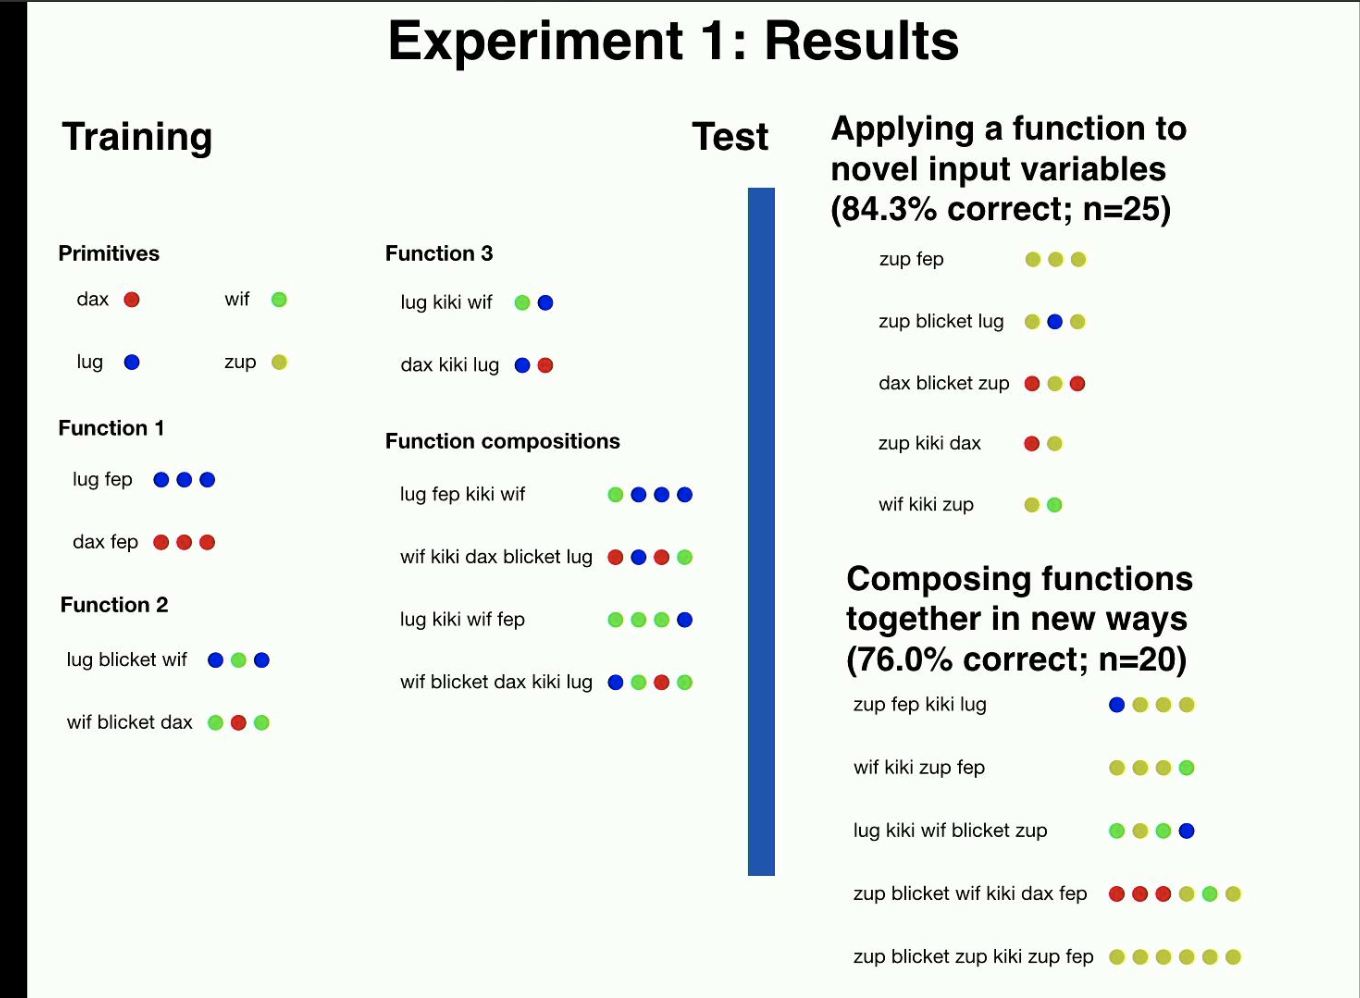
\includegraphics[width=0.42\textwidth]{figures/dax_blicket.png}}
    \subfloat[Inductive Biases]{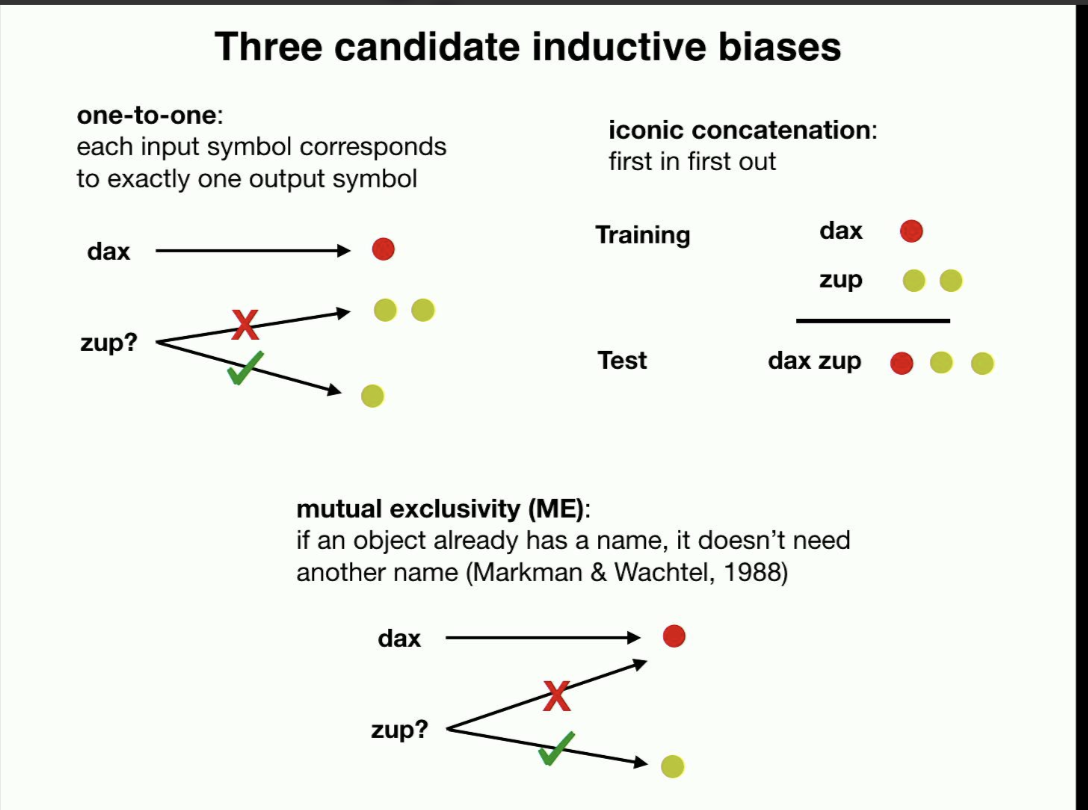
\includegraphics[width=0.42\textwidth]{figures/ind_bias.png}}
    \caption{Some examples from the dataset (left) and visuals of inductive biases (right).}
    \label{fig:blicket}
\end{figure}

Summary: find several inductive biases in participants such as $\ra$ 1) one-to-one: people like these mappings, 2) iconic concatenation(first in first out), and 3) mutual exclusivity: everything has {\it one} name, not more. \\

Experiment 2: free-form prompts, examine inductive biases on seq2seq task with NO training examples. \\

$\ra$ More than a source of error, these biases provide critical inductive constraints. \\

Central Q: Can compositional skills be acquired through meta-learning? \\

Goals:
\begin{itemize}
    \item Want a structured neural network that can:
    \begin{itemize}
        \item Learn new primitives and use the compositionality
        \item Encode inductive biases
        \item Capture rich starting point people bring to compositional learning tasks
    \end{itemize}
    \item Do NOT intend models to explain developmental process, resolve which components are learned vs. innate.
\end{itemize}

New work that tries to capture the above goals: Meta sequence-to-sequence learning \cite{lake2019compositional}.
\begin{itemize}
    \item Learning is distributed over a series of dynamically changing datasets that encourage compositional generalization
    \item Training episodes contain thousands of support/query set.
    \item No weight updates at test set.
    
    \item Architecture has RNN encoders for the support, passed with attention to a decoder.
    
    $\ra$ But, meaning of words is changing between episodes! So can't learn a fixed mapping.
\end{itemize}

Q: Can a network acquire human-like biases? \\

A: Yes, it seems! Results: achieved 100\% on quickly acquiring new mappings. \\

$\ra$ Also applied to SCAN: evaluated on new episodes with original mappings. Meta seq2seq achieves 99.95\% on adding ``jump" (the piece that broke earlier models). \\

Coming back to ``dax": both people and the model can learn a new verb and use it compositionally. Model needs to see a lot of combinations of similar pairs, though. \\

{\bf A Step Back:}
\begin{enumerate}
    \item Wanted a framework that can:
\begin{itemize}
\item Learn new primitives and use the compositionality
        \item Encode inductive biases
        \item Capture rich starting point people bring to compositional learning tasks
\end{itemize}
\item We now have those three properties!
\item Lots to do though: 1) modeling details of human behavior, 2) acquire human priors, 3) Learn new primitives, 4) Understand how these abilities develop, 5) Large scale compositional word learning.
\end{enumerate}

Started with the question: ``what are the computational underpinning of human compositional skills?" Studied:
\begin{enumerate}
    \item Powerful seq2seq models fail spectacularly when systematic compositional skills are required
    \item People can learn new concepts and apply them in new ways
    \item Structured, memory-augmented networks can perform few shot composition.
\end{enumerate}

Challenge Question: How do we know what the right inductive biases are? \\

Brenden Lake: We should look to cognitive development! Early emerging abilities are likely to be most important. We should study computational problems that are easier fr people than for machines. Collect behavioral data and reverse engineer human inductive biasers. I see meta learning as a tool for encoding priors in cognitive modeling or machin learning that are too difficult to specify by hand or easier to specify in data than an explicit prior. In the Bayesian sense, we want a put a prior on our model but it's hard to specify: meta-learning can be an effective way to specify complex priors. \\

\dnote{And that's a wrap! I'm doing the panel now.}

